\documentclass{report}
\usepackage{xcolor}
\usepackage{listings}
\usepackage{amsmath,amssymb,graphicx,graphics,caption}
\usepackage{svg}

%\newcommand*{\conceptfont}{\fontfamily{pcr}\selectfont}
%\DeclareTextFontCommand{\conceptfont}{pcr}
\newcommand{\concept}[1]{\fontfamily{pcr}{\selectfont #1}}

\lstdefinestyle{dsl}
{
  language=python, 
  keywordstyle=\color{red}, 
  commentstyle=\color{blue}, 
  morekeywords={forall},   keywordstyle=\color{red},        
  numbers=left, numberstyle=\tiny, stepnumber=1, numbersep=5pt,
  classoffset=1,
  morekeywords={computation, field, imap, op},   keywordstyle=\color{purple}
}


\begin{document}

\section*{Overview of GungHO/LFRic Data Structures}

\section{Mesh}

LFRic mesh is unstructured in the horizontal and structured in vertical. This means that
it is enough to enough to store the coordinates and connectivity information for a 
single horizontal level (horizontal 2D mesh) and infer coordinates of all levels 
from this information.

\subsection{Global 2D Mesh}

Described by
\begin{itemize}
\item \concept{Vertex} (coordinates of a single mesh vertex),
\item \concept{Connectivity} (topology defined by the list of connections between pairs of vertices)
\end{itemize}

\concept{Connectivity} is further described by
\begin{itemize}
\item \concept{FaceNodeConnectivity} (vertices which form each cell),
\item \concept{EdgeNodeConnectivity} (vertices found on each edge),
\item \concept{FaceEdgeConnectivity} (edges found on each cell),
\item \concept{FaceFaceConnectivity} (id of each cell to which the index cell is adjacent).
\end{itemize}

Global mesh is created by a mesh generator for specific domain (Cartesian 
biperiodic or cubed sphere, see Fig.~\ref{fig:cube_sphere_layout} for the latter). 
The connectivity information is stored as lookup tables.

\begin{figure}
\begin{centering}
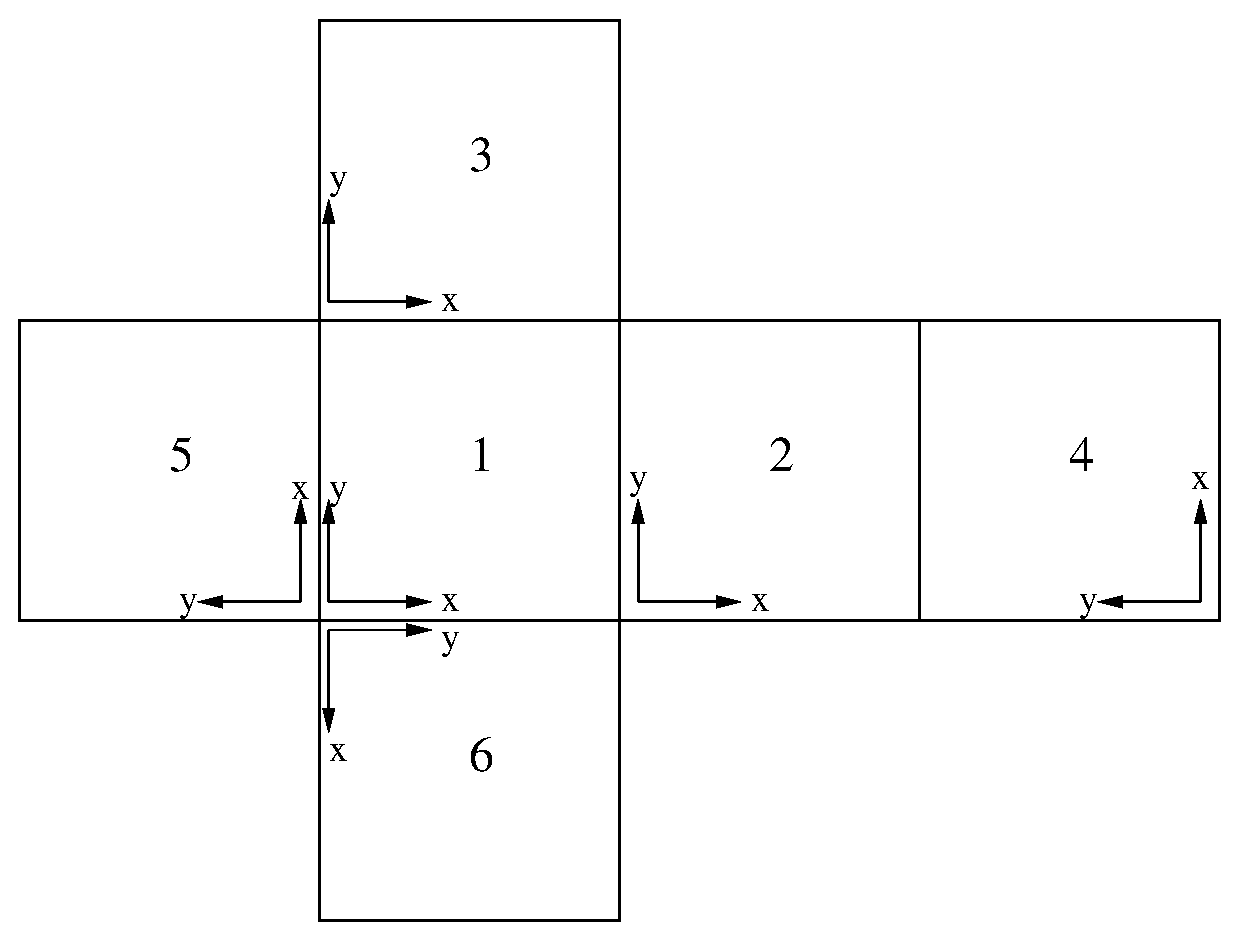
\includegraphics[scale=0.5]{lfricdoc_figures/cube_layout.eps}
\protect\caption{\label{fig:cube_sphere_layout}Layout of the cube sphere faces showing
the panel local coordinate directions so that there is no change in
orientation of normal or tangent directions between panels.}
\par\end{centering}
\end{figure}

\subsection{Partition}

Local meshes are created for each partition of a distributed memory configuration
by applying mesh-type dependent partitioning strategy (currently cubed-sphere or biperiodic mesh)
to the 2D global mesh and extruding in the vertical direction.

Partition class is described by
\begin{itemize}
\item \concept{InnerCells} (cells that are inner partition halo cells),
\item \concept{EdgeCells} (cells that are owned by the partition but may have dofs that are also owned by halo cells),
\item \concept{HaloCells} (cells that are halo cells),
\item \concept{GhostCells} (cells in an extra halo around the outermost actual halo and are not in the partitioned domain, but are required to fully describe the cells in the partitioned domain),
\item \concept{LocalRank} (local distributed memory rank number),
\item \concept{TotalRanks} (total number of distributed memory ranks),
\item \concept{GlobalCellID} (global IDs of all cells in local partition).
\end{itemize}

This allows strategies such as concurrent communication and computation to be applied.

\subsection{Local 3D Mesh}

As said above, coordinates of vertical levels can inferred from coordinates of a single
horizontal level 2D mesh by adding 1 to the addresses
of the values of the cell on the level below so only storing the look-up array that
addresses cells on the lowest level is required. 
The extrusion of the 2D mesh into a 3D mesh extends the list
of mesh entities.

\begin{itemize}
\item \concept{Vertices} (a vertical column of vertices all at the same latitude and longitude of the 2D mesh),
\item \concept{Edges}
  \begin{itemize}
  \item \concept{VerticalEdge} (connect the vertices with the same latitude and longitude on each adjacent height level),
  \item \concept{HorizontalEdge} (connect vertices as in the 2D example on each layer of the 3D mesh),
  \end{itemize}
\item \concept{Faces}
  \begin{itemize}
  \item \concept{VerticalFace} (2D faces between an edge on one height level and the corresponding edge on the next),
  \item \concept{HorizontalFace} (as the original 2D faces/cells description except there is a set of horizontal faces on each level),
  \end{itemize}
\item \concept{Cells} (3D elements created by the extrusion of the 2D face into 3D).
\end{itemize}

\begin{figure}
\begin{centering}
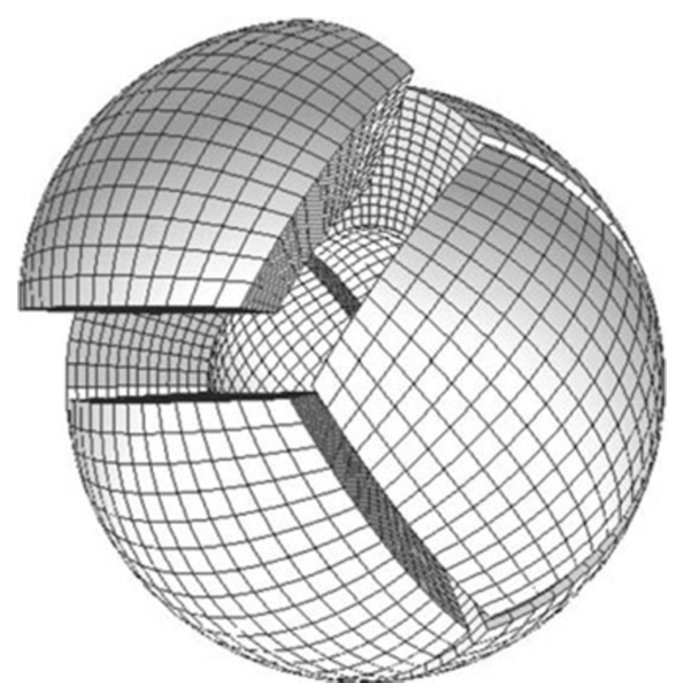
\includegraphics[scale=0.5]{lfricdoc_figures/cubed_sphere.eps}
\protect\caption{\label{fig:cubed_sphere}A 3-dimensional cubed sphere mesh, taken apart to see the levels structure.}
\par\end{centering}
\end{figure}

\section{Function Space}

GungHo mixed FEM formulation employs different discretisations to represent
different quantities. This means that the data points are not collocated. 
GungHo function spaces, called ($\mathbb{W}_0$), ($\mathbb{W}_1$), ($\mathbb{W}_2$) 
and ($\mathbb{W}_3$), aremathematically related as follows.

\begin{equation}
\begin{array}{ccccccc}
\mathbb{W}_{0} & \overset{\nabla}{\longrightarrow} & \mathbb{W}_{1} & \overset{\nabla\times}{\longrightarrow} & \mathbb{W}_{2} & \overset{\nabla.}{\longrightarrow} & \mathbb{W}_{3}\\
 & \underset{\tilde{\nabla.}}{\dashleftarrow} &  & \underset{\tilde{\nabla}\times}{\dashleftarrow} &  & \underset{\tilde{\nabla}}{\dashleftarrow}
\end{array}\label{eq:derham_complex}
\end{equation}

Each function space can be created at {\em lowest order} (constant and linear functions) 
or at increasingly {\em higher order} (where constant functions become linear, linear become
quadratic and so forth). Placement of {\em degrees of freedom} ("dofs") for the four main
function spaces is in Fig.~\ref{fig:k0k1w0-w3}. They can share dofs between cells in
horizontal, vertical or both directions. 

%
\begin{figure}
\begin{minipage}{.5\textwidth}
  \centering
  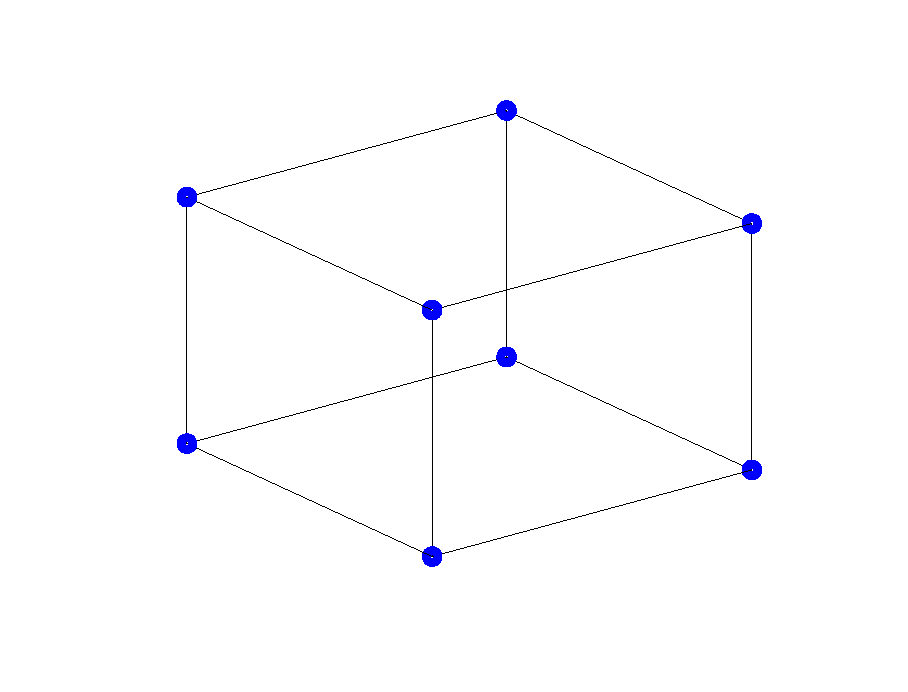
\includegraphics[width=0.7\linewidth]{lfricdoc_figures/k0_W0_dofs.eps}
  \captionof*{figure}{a) $\mathbb{W}_{0}, k = 0$}
  \label{fig:k0w0}
\end{minipage}%
\begin{minipage}{.5\textwidth}
  \centering
  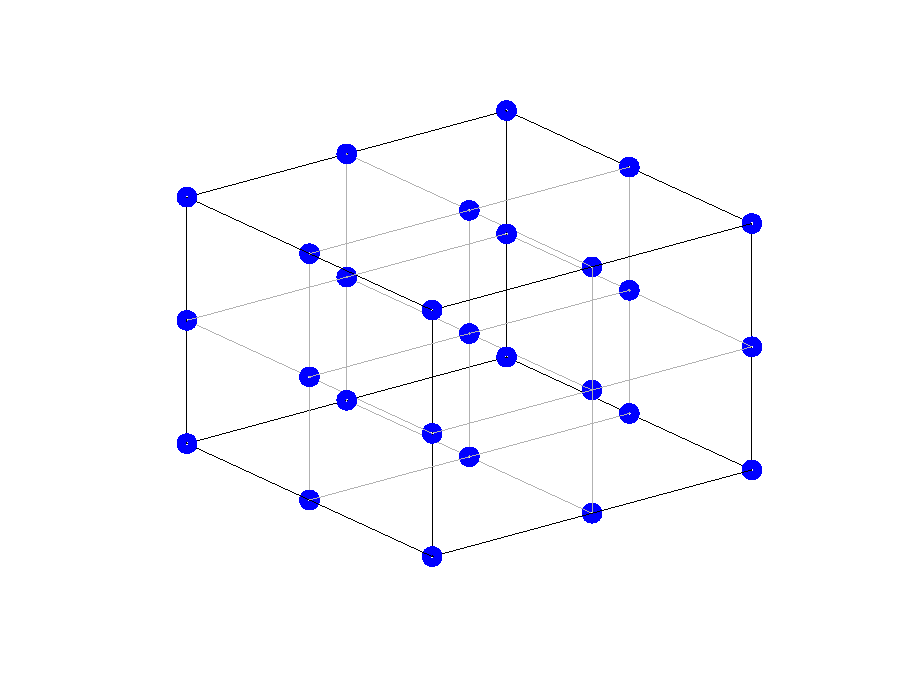
\includegraphics[width=0.7\linewidth]{lfricdoc_figures/k1_W0_dofs.eps}
  \captionof*{figure}{b) $\mathbb{W}_{0}, k = 1$}
  \label{fig:k0w02}
\end{minipage}

\begin{minipage}{.5\textwidth}
  \centering
  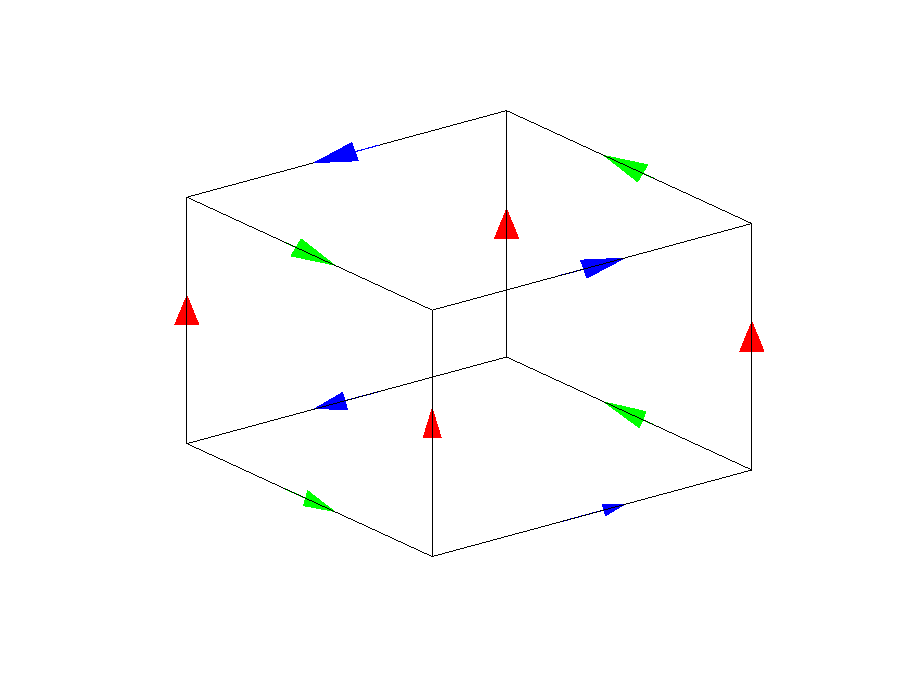
\includegraphics[width=0.7\linewidth]{lfricdoc_figures/k0_W1_dofs.eps}
  \captionof*{figure}{c) $\mathbb{W}_{1}, k = 0$}
  \label{fig:k0w1}
\end{minipage}%
\begin{minipage}{.5\textwidth}
  \centering
  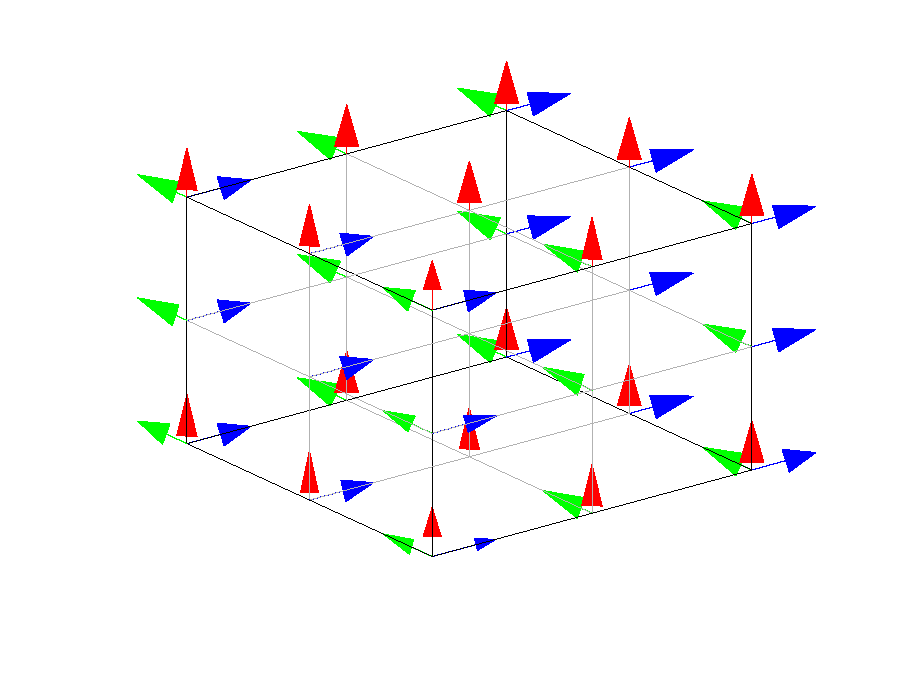
\includegraphics[width=0.7\linewidth]{lfricdoc_figures/k1_W1_dofs.eps}
  \captionof*{figure}{d) $\mathbb{W}_{1}, k = 1$}
  \label{fig:k1w1}
\end{minipage}

\begin{minipage}{.5\textwidth}
  \centering
  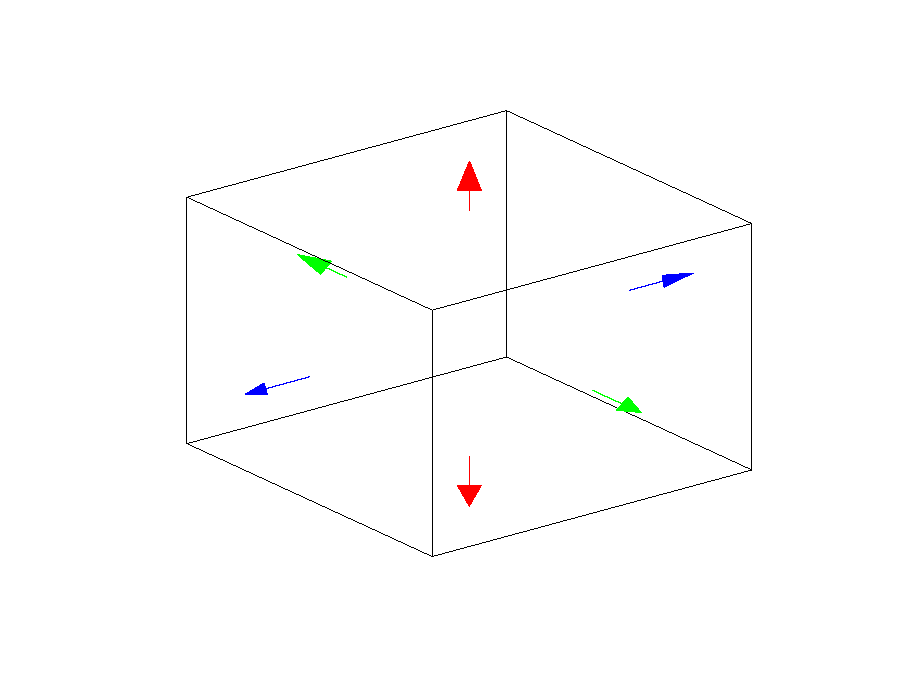
\includegraphics[width=0.7\linewidth]{lfricdoc_figures/k0_W2_dofs.eps}
  \captionof*{figure}{e) $\mathbb{W}_{2}, k = 0$}
  \label{fig:k0w2}
\end{minipage}%
\begin{minipage}{.5\textwidth}
  \centering
  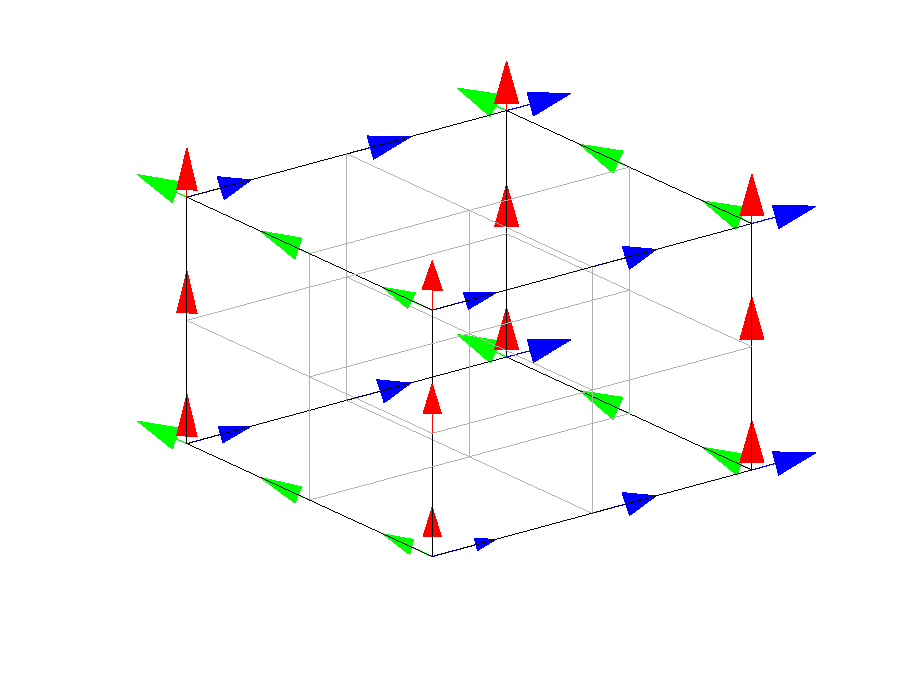
\includegraphics[width=0.7\linewidth]{lfricdoc_figures/k1_W2_dofs.eps}
  \captionof*{figure}{f)$\mathbb{W}_{2}, k = 1$}
  \label{fig:k1w2}
\end{minipage}

\begin{minipage}{.5\textwidth}
  \centering
  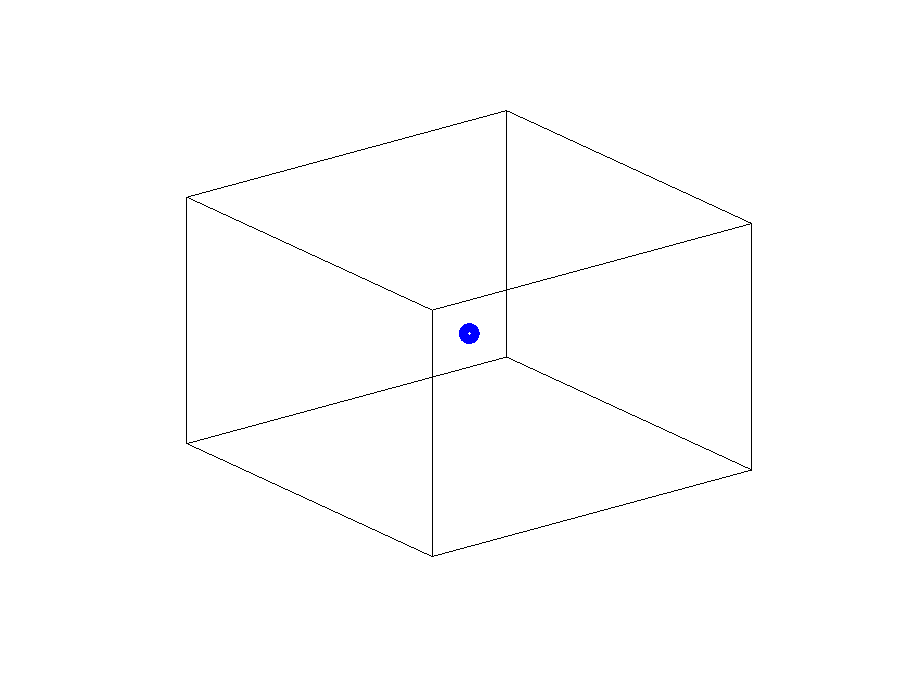
\includegraphics[width=0.7\linewidth]{lfricdoc_figures/k0_W3_dofs.eps}
  \captionof*{figure}{g) $\mathbb{W}_{3}, k = 0$}
  \label{fig:k0w3}
\end{minipage}%
\begin{minipage}{.5\textwidth}
  \centering
  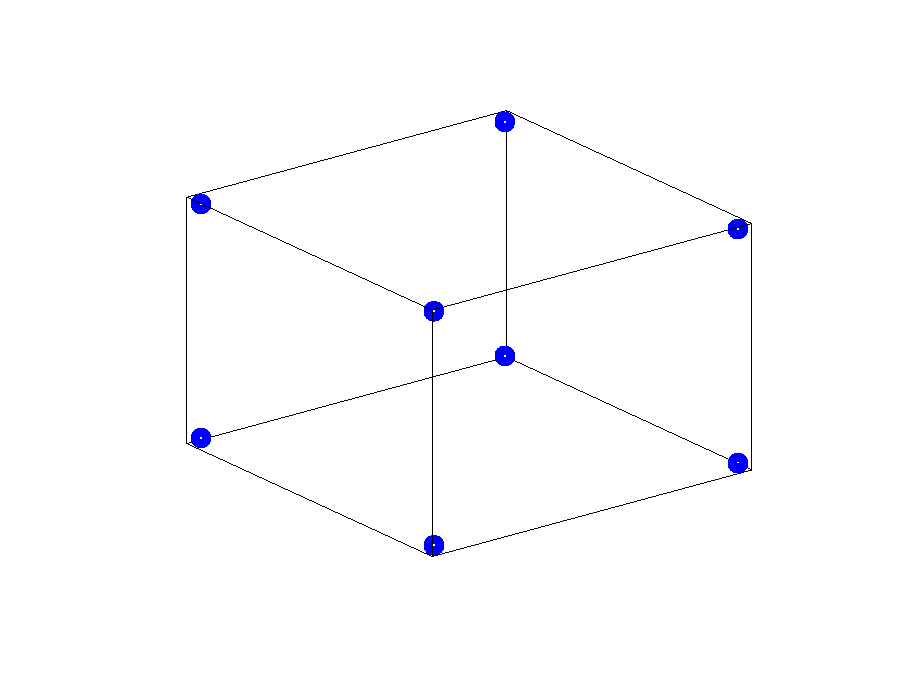
\includegraphics[width=0.7\linewidth]{lfricdoc_figures/k1_W3_dofs.eps}
  \captionof*{figure}{h) $\mathbb{W}_{3}, k = 1$}
  \label{fig:k1w3}
\end{minipage}

\caption{Locations of dofs for spaces $\mathbb{W}_0$ to $\mathbb{W}_3$
  for lowest order in left column, and next lowest in right.}
\label{fig:k0k1w0-w3}
\end{figure}

The function space instance is created for a given mesh, order and continuity. 
Each distributed memory rank creates a function space instance for its own local partition.
Function spaces are described by:
\begin{itemize}
\item \concept{Dofmap} (holds the indirection map, i.e.\ the dofmap for the first level of cells of the 3D mesh),
\item \concept{GlobalID} (the number and location of degrees of freedom within the whole 3-dimensional extent of the local
mesh).
\item \concept{Basis} (functions to evaluate the basis functions),
\item \concept{DiffBasis} (functions to evaluate the differentials of basis functions),
\item \concept{DofRange} (functions to access the range of dofs in different parts of the local field, such as those within a
given halo).
\end{itemize}

Function space instance also contains functions to access information about the mesh, such as its colouring strategy.


\vspace{12pt} Dofmaps can be set up to list any groupings of dofs over mesh entities: 
\begin{itemize}
\item \concept{VolumeDofmap} (stores the dofs in a cell volume),
\item \concept{EdgeDofmap} (stores the dofs on cell edges),
\item \concept{FaceDofmap} (stores the dofs on cell faces),
\item \concept{VertexDofmap} (stores the dofs on cell vertices),
\end{itemize}
so the application can loop over one or more of these groups. 

LFRic utilises the \concept{CellDofmap} which stores all these dofs 
(dofs in a cell volume plus the dofs on the faces, edges and vertices
on the boundary of the cell)


The ordering of the dofs within the cell dofmap is dofs on (1) volumes, 
(2) faces, (3) edges and (4) vertices. The ordering of faces, edges and 
vertices is given by the reference element for each function space.

For example, the cell dofmap applied to a velocity field on function space $\mathbb{W}_{2}$ and
lowest element order ($k=0$) for cell \texttt{i} will return (see Fig.~\ref{fig:k0k1w0-w3}e)

\begin{minipage}[t]{1\columnwidth}%
\smallskip

\texttt{dofmap\_w2(:,i)={[}u\_face1,u\_face2,u\_face3,u\_face4,u\_face5,u\_face6{]}.}
\smallskip

\end{minipage}

This is equivalent to placement of velocity
components on a C-grid finite difference model for a cell located at 
$\left(i-\frac{1}{2},k-\frac{1}{2},k-\frac{1}{2}\right)$:

\begin{minipage}[t]{1\columnwidth}%
\smallskip

\texttt{dofmap\_endgame(:,i,j,k)=
\newline{[}$u_{i-1,j-\frac{1}{2},k-\frac{1}{2}},u_{i,j-\frac{1}{2},k-\frac{1}{2}},v_{i-\frac{1}{2},j-1,k-\frac{1}{2}},v_{i-\frac{1}{2},j,k-\frac{1}{2}},w_{i-\frac{1}{2},j-\frac{1}{2},k-1},w_{i-\frac{1}{2}.j-\frac{1}{2},k}${]}.}
\par

\smallskip

\end{minipage}

\subsection{Reference Element}

Contains the topology of a reference element, a unit cell, in order to implement placement of the 
dofs for each function space. Includes ordering of topological entities and lookups for dofs on a unit cell.

\begin{itemize}
\item \concept{Coordinates}
  \begin{itemize}
  \item \concept{VertexCoordinates} (coordinates of the vertices relative to a unit cell),
  \item \concept{EdgeCoordinates} (coordinates of the edges relative to a unit cell),
  \item \concept{FaceCoordinates} (coordinates of the faces relative to a unit cell),
  \item \concept{VolumeCoordinates} (coordinates of the volume centres relative to a unit cell),
  \end{itemize}
\item \concept{Connectivity}
  \begin{itemize}
  \item \concept{VertexOnFace} (vertices around one face),
  \item \concept{VertexOnEdge} (vertices on one edge),
  \item \concept{EdgeOnFace} (edges around one face),
  \item \concept{EdgeOnVert} (edges around one vertex),
  \item \concept{FaceOnEdge} (faces around one edge).  
  \end{itemize}
\end{itemize}

\section{Field}

Fields represent FEM discretisations of various prognostic and diagnostic variables
and as such utilise the previously described structures.

Field values at points within a cell are evaluated as the sum of a set of basis functions 
multiplied by coefficients which are located in the data points (dofs) for a specific 
function space. Points of evaluation are determined by a quadrature object and are 
independent of the function space the field is on.

As mentioned in function space description, a field can have mixed continuity in the
horizontal and vertical directions. Additionally, fields on vector function spaces 
($\mathbb{W}_{1}$ and $\mathbb{W}_{2}$) may have different continuity for vector 
components (e.g. continuous normal to a face between two cells but discontinuous 
parallel to the face in case of $\mathbb{W}_{2}$).

\end{document}
